\documentclass{article}

% Language setting
% Replace `english' with e.g. `spanish' to change the document language
\usepackage[english]{babel}
\usepackage{minted}

\usepackage[utf8]{inputenc}
\usepackage{array}
\usepackage{float}

\usepackage[letterpaper,top=2cm,bottom=2cm,left=3cm,right=3cm,marginparwidth=1.75cm]{geometry}

% Useful packages
\usepackage{amsmath}
\usepackage{graphicx}
\usepackage[colorlinks=true, allcolors=blue]{hyperref}

\title{ME-489 HOMEWORK 6 REPORT}
\author{Alperen Çalışkan & Ali Taha Akpınar}

\begin{document}
\definecolor{mygray}{rgb}{0.95,0.95,0.95}
\setminted[c]{autogobble=true, frame=lines, framesep=4mm, baselinestretch=1.2,
bgcolor=mygray, fontsize=\footnotesize,linenos=true}
\setminted[latex]{autogobble=true, frame=lines, framesep=4mm, baselinestretch=1.2,
bgcolor=mygray, fontsize=\footnotesize,linenos=true}
\maketitle
\begin{abstract}
In this report the paralelized code of the serial Mandelbrot set code explained. The Mandelbrot set is a set created by using complex numbers and their squares. The instructor of the course has provided us with the serial code for the Mandelbrot set. For this homework, unlike the previous homeworks, the GPU is parallelized using CUDA and Google Colab environment.
\end{abstract}

\section{Introduction}
The Mandelbrot set is a well known set among mathematicians and computer scientiest for some time. The set defines a complex field. For any point in the field it is checked whether the point is stable when the following relation is aplied. The relation states that for the complex number z, if it z is squared and summed with a constant for many times until it reaches a stable number or not. To get the Mandelbrot set the starting point should be 0. In essence this set is a useful visualisation when trying to see where the following relation is stable or not.
\begin{align*}
z_0 &= 0 \\
z_{n+1} &= z_n^2 + c
\end{align*}
The black part in the set correspond to stability. 

\section{GPU implementation}
The serial code is working well. The serial code is parallelised with CUDA implementation. There are a total 4096*4096 pixel calculations. For each of the calculations one thread is created. One block has at most 1024 threads and the amount of blocks are within the wanted range. In the code every block has 2 dimensions and the grşd also has 2 dimensions. The dimensions are created as follows:
\begin{minted}{c}
dim3 block_dim(p_w, p_w, 1);
dim3 grid_dim(((Nre + p_w - 1 )/p_w),((Nim + p_w - 1 )/p_w), 1);
\end{minted}
For the structs cmin and dc, two other structs are created into the device named d\_cmin and d\_dc.
\begin{minted}{c}
  cudaMalloc((void **)&d_cmin, sizeof(complex_t));
  cudaMalloc((void **)&d_dc, sizeof(complex_t));
  cudaMemcpy(d_cmin, &cmin, sizeof(complex_t), cudaMemcpyHostToDevice);
  cudaMemcpy(d_dc, &dc, sizeof(complex_t), cudaMemcpyHostToDevice);
\end{minted}
Also for the count array another array is created and copied to the device:
\begin{minted}{c}
float *count;
count = (float*) malloc(Nre*Nim*sizeof(float));
float *d_count;
cudaMalloc((void**)&d_count,Nre*Nim*sizeof(float));
cudaMemcpy(d_count, count, Nre * Nim * sizeof(float), cudaMemcpyHostToDevice);
\end{minted}
Kernel is called using the following:
\begin{minted}{c}
mandelKernel<<<grid_dim, block_dim>>>(Nre, Nim, d_cmin, d_dc, d_count);
\end{minted}
After the kernel is called the device count array is copied back to the host count array.
\begin{minted}{c}
cudaMemcpy(count, d_count, Nre * Nim * sizeof(float), cudaMemcpyDeviceToHost);
\end{minted}
\subsection{\_\_global\_\_ void mandelKernel}
The x and y coordinates for the pixels are determined for each thread as follows:
\begin{minted}{c}
int m = blockIdx.x * blockDim.x + threadIdx.x;
int n = blockIdx.y * blockDim.y + threadIdx.y;
\end{minted}
The threads should stop calculating the counted value after it is over the Nre and Nim numbers.
\begin{minted}{c}
  if(m<Nre && n<Nim){
    complex_t c;
    c.x = d_cmin->x + d_dc->x*m;
    c.y = d_cmin->y + d_dc->y*n;
    d_count[m+n*Nre] = (float) testpoint(c);
    }
\end{minted}

In order to make testpoint available to device \_\_device\_\_ title is added to it.
\section{Scaling}
\subsection{With 4096*4096 pixels}
With the serial code the following results are attained:
\begin{minted}{c}
elapsed = 24.570002
\end{minted}
When there are 2 by 2 threads for each block
\begin{minted}{c}
elapsed = 2.055222 seconds
\end{minted}
When there are 4 by 4 threads for each block
\begin{minted}{c}
elapsed = 0.662374 seconds
\end{minted}
When there are 8 by 8 threads for each block
\begin{minted}{c}
elapsed = 0.459941 seconds
\end{minted}
When there are 16 by 16 threads for each block
\begin{minted}{c}
elapsed = 0.454190 seconds
\end{minted}
When there are 32 by 32 threads for each block
\begin{minted}{c}
elapsed = 0.469859 seconds
\end{minted}

\subsection{With 8192*8192 pixels}
With the serial code the following results are attained:
\begin{minted}{c}
elapsed = 89.078839
\end{minted}
When there are 2 by 2 threads for each block
\begin{minted}{c}
elapsed = 7.480773 seconds
\end{minted}
When there are 4 by 4 threads for each block
\begin{minted}{c}
elapsed = 2.185179 seconds
\end{minted}
When there are 8 by 8 threads for each block
\begin{minted}{c}
elapsed = 1.334092 seconds
\end{minted}
When there are 16 by 16 threads for each block
\begin{minted}{c}
elapsed = 1.302079 seconds
\end{minted}
When there are 32 by 32 threads for each block
\begin{minted}{c}
elapsed = 1.301523 seconds
\end{minted}
\section{Conclusion}
This report discusses a detailed parallelization of the Mandelbrot set code using CUDA. The Mandelbrot set, a complex field, was analyzed through a stability relation, and the serial code was successfully parallelized with GPU implementation. Scaling experiments with different pixel sizes further confirmed the advantages of parallelization in reducing computation time.
It is evident that the time it takes for calculating all the pixel counts decreases significantly when parallelization is applied. It is also clear that as the number of threads in each block increased, the time also increased until 32 by 32 threads per block. In summary, parallelizing the Mandelbrot set code using CUDA proved to be a successful strategy for optimizing performance. The obtained image is below:
\begin{figure}[h!]
\centering
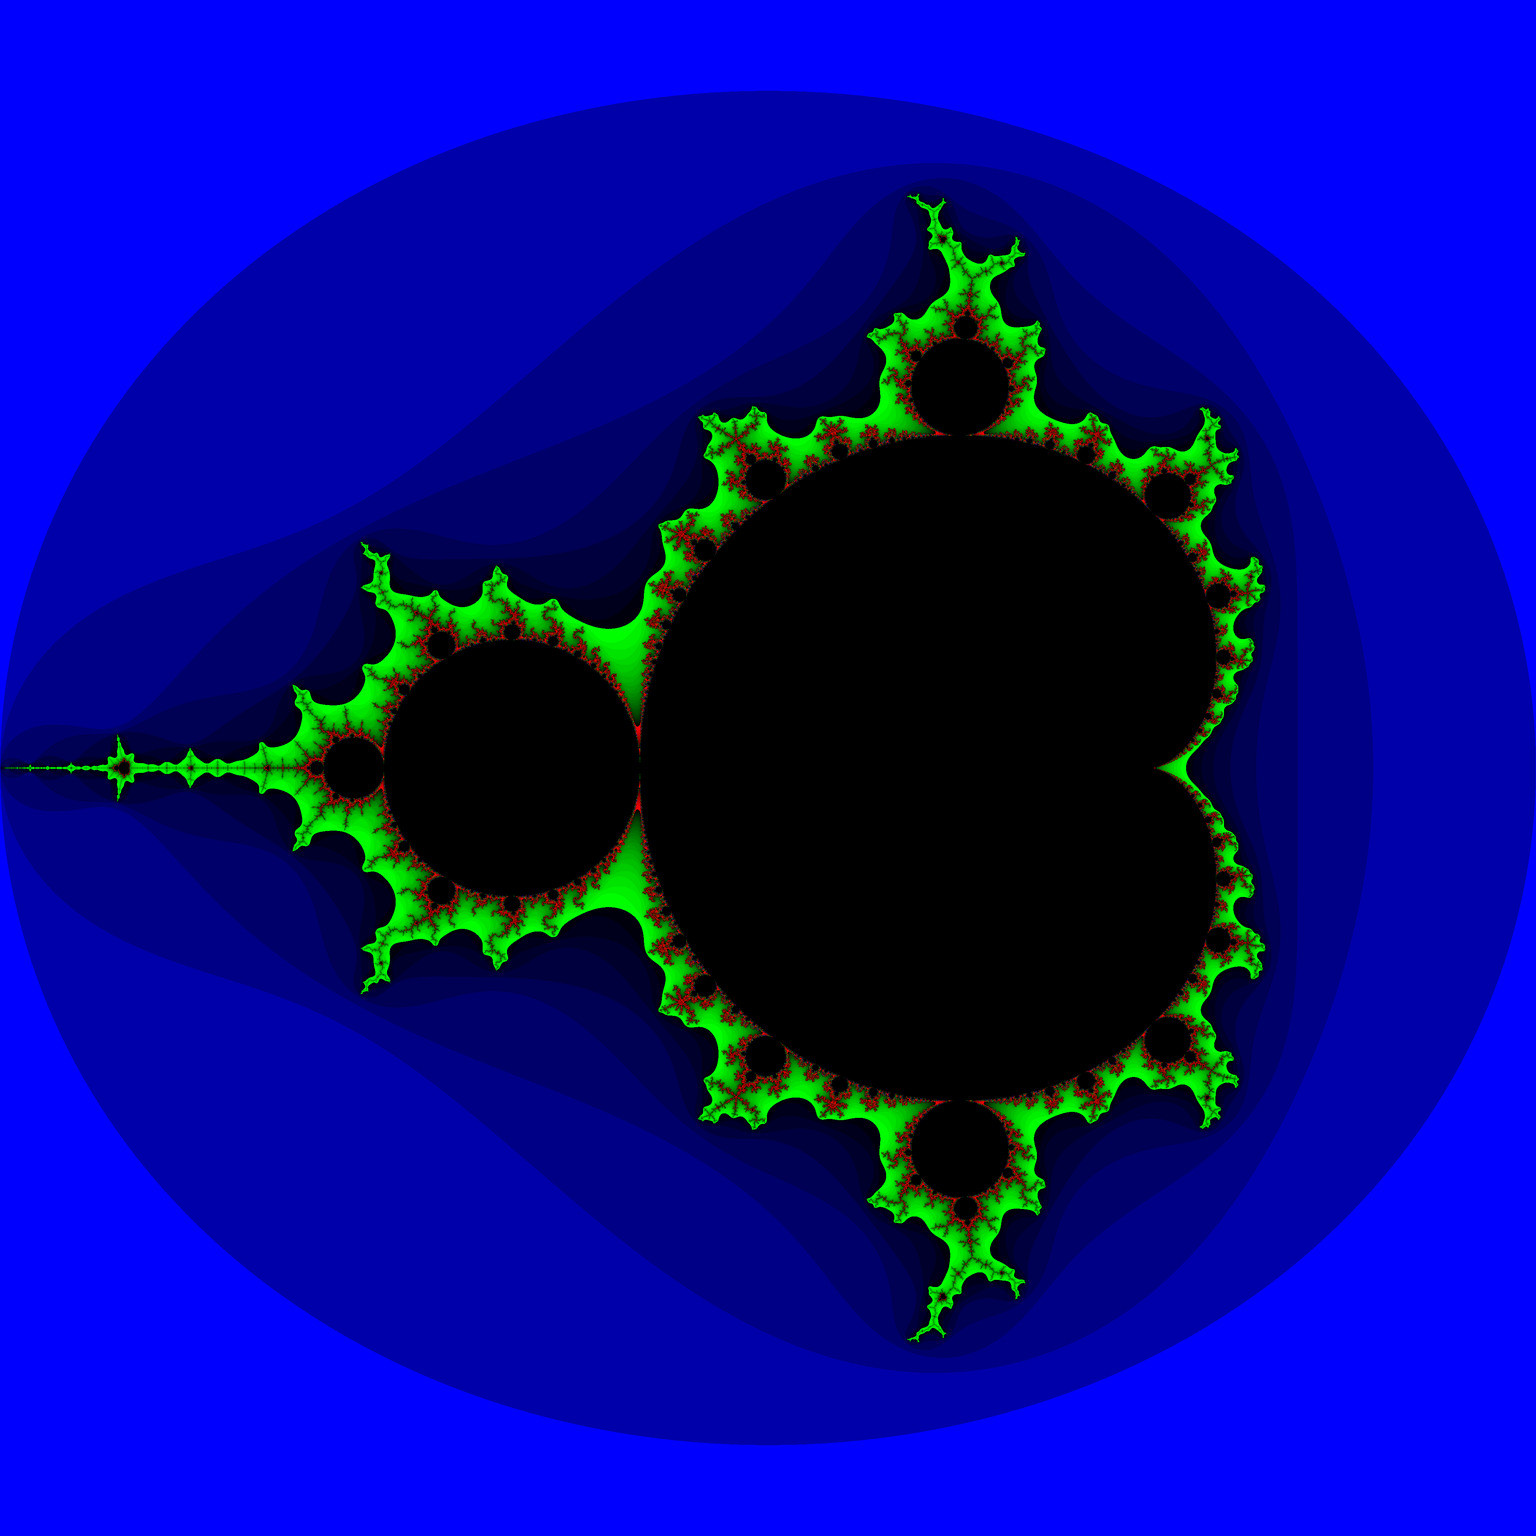
\includegraphics[width=0.60\linewidth]{mandelbrot.jpg}
\caption{\label{fig:Mandelbrot Set}This is the colorized Mandelbrot set obtained with escape time algorithm. }
\end{figure}
\end{document}